We provide several coordination facts for dealing with node partitioning among
the running threads. Since each node is placed in some thread, the partitioning
facts revolve around thread placement.  In terms of action facts, we have the
following:

\begin{itemize}
   \item \code{set-thread(node A, thread T)}: Moves node \code{A} to thread
      \code{T} and forces \code{A} to be in \code{T} indefinitely.

   \item \code{set-affinity(node A, node B)}: Places node \code{B} in the thread
      of node \code{A} and forces \code{B} to be in the thread indefinitely.

   \item \code{set-moving(node A)}: Allows node \code{A} to move freely
   between threads.

\end{itemize}

As an example of \code{set-thread}, consider again the graph in
Fig.~\ref{fig:coordination:priorities}. If a coordination fact
\code{set-thread(@2, T1)} is derived, then node \code{@2} will become part
of the sub-graph of thread \code{T1}. The result is shown in
Fig.~\ref{fig:coordination:partitioning}.

\begin{figure}
\begin{center}
   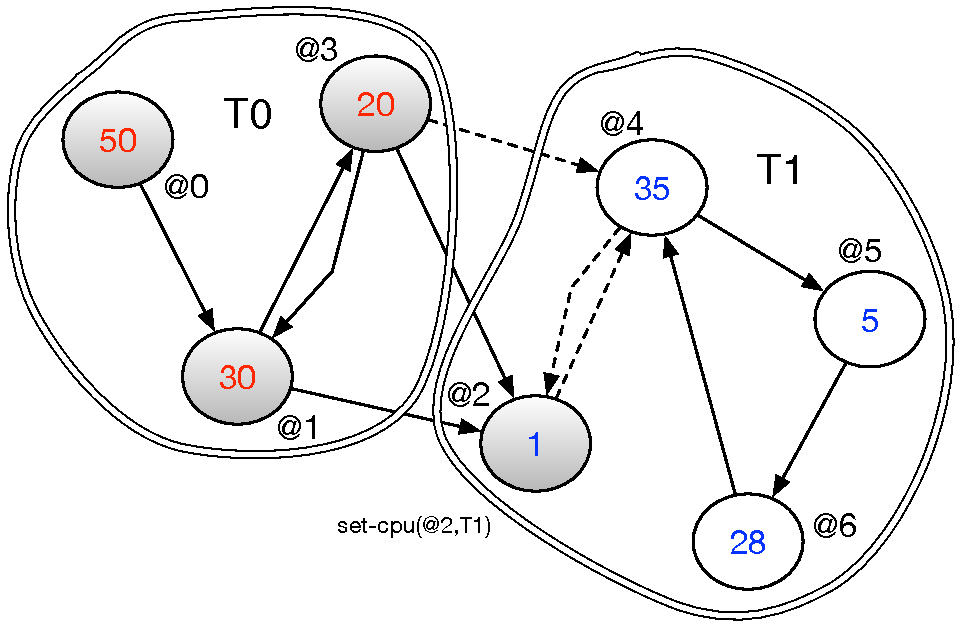
\includegraphics[width=0.6\textwidth]{figures/coordination/partitioning.pdf}
\end{center}
\caption{Moving node \code{@2} to thread \code{T1} using
   \code{set-thread(@2, T1)}.}
\label{fig:coordination:partitioning}
\end{figure}

Sensing facts retrieve information about node placement and are specified as
follows:

\begin{itemize}

   \item \code{thread-id(node A, thread T)}: Linear fact that maps node \code{A}
      to thread \code{T} which \code{A} belongs to. Fact \code{set-thread}
      implicitly updates fact \code{thread-id}.

   \item \code{is-static(node A)}: Fact available at node \code{A} if
      \code{A} is not allowed to move between threads.

   \item \code{is-moving(node A)}: Fact available at node \code{A} if
      \code{A} is allowed to move between threads.

   \item \code{just-moved(node A)}: Linear fact derived by the
      \code{set-thread} action if, at that moment, the node \code{A} is running
      on the target thread.

\end{itemize}

